\subsection*{1.标准状态:灯丝电源电压{{v_lamp_1}}v,$V_{G1K}$电压{{v_g1k_1}}v,$V_{G2A}$电压{{v_g2a_1}}v,$V_{G2K}$电压{{v_g2k_1}}v}
\begin{center}
\begin{tabular}{|c|c|c|c|c|c|c|}
	\hline
	波峰&V1&V2&V3&V4&V5&V6
	\\\hline
	电压/V
	
		&{{a}}
	
	\\\hline
	\end{tabular}
	\end{center}

$$  \bar{V_0}=\frac{V_4+V_5+V_6-V_3-V_2-V_1}{3\times 3}={{ave_v0_1}}V $$
$$	\Delta V_1=\frac{1}{3}(V_4-V_1)={{del_v1_1}}V $$
$$	\Delta V_2=\frac{1}{3}(V_5-V_2)={{del_v2_1}}V $$
$$	\Delta V_3=\frac{1}{3}(V_6-V_3)={{del_v3_1}}V $$ 

\ \\
A类不确定度:
$$	u_a(V_0)=\sqrt{\frac{\sum\limits_{i=1}^{3} (\Delta V_i-\bar{V_0})^2}{3\times 2}}={{ unc_a_1 }}V $$
B类不确定度:
$$	u_b(V_0)=\frac{0.1V}{\sqrt{3}}=0.058V $$
不确定度:
$$	u(V_0)=\sqrt{u_a(V_0)_2+u_b(V_0)_2}={{unc_s_1}}V $$
相对不确定度:
$$	\eta=\frac{u(V_0)}{V_0}={{unc_r_1}} $$
最终结果为:
$$	V_0 \pm u(V_0) = ({{ave_v0_1}} \pm {{ unc_s_1}})V $$


\subsection*{2.灯丝电源电压改变为${{v_lamp_2}}$v}
\begin{center}
\begin{tabular}{|c|c|c|c|c|c|c|}
	\hline
	波峰&V1&V2&V3&V4&V5&V6
	\\\hline
	电压/V
	
		&{{a}}
	
	\\\hline
	\end{tabular}
	\end{center}

$$  \bar{V_0}=\frac{V_4+V_5+V_6-V_3-V_2-V_1}{3\times 3}={{ave_v0_2}}V $$
$$	\Delta V_1=\frac{1}{3}(V_4-V_1)={{del_v1_2}}V $$
$$	\Delta V_2=\frac{1}{3}(V_5-V_2)={{del_v2_2}}V $$
$$	\Delta V_3=\frac{1}{3}(V_6-V_3)={{del_v3_2}}V $$ 

\ \\
A类不确定度:
$$	u_a(V_0)=\sqrt{\frac{\sum\limits_{i=1}^{3} (\Delta V_i-\bar{V_0})^2}{3\times 2}}={{ unc_a_2 }}V $$
B类不确定度:
$$	u_b(V_0)=\frac{0.1V}{\sqrt{3}}=0.058V $$
不确定度:
$$	u(V_0)=\sqrt{u_a(V_0)_2+u_b(V_0)_2}={{unc_s_2}}V $$
相对不确定度:
$$	\eta=\frac{u(V_0)}{V_0}={{unc_r_2}} $$
最终结果为:
$$	V_0 \pm u(V_0) = ({{ave_v0_2}} \pm {{ unc_s_2}})V $$


\subsection*{3.$V_{G1K}$ 电压改变为${{v_g1k_3}}$v}
\begin{center}
\begin{tabular}{|c|c|c|c|c|c|c|}
	\hline
	波峰&V1&V2&V3&V4&V5&V6
	\\\hline
	电压/V
	
		&{{a}}
	
	\\\hline
	\end{tabular}
	\end{center}

$$  \bar{V_0}=\frac{V_4+V_5+V_6-V_3-V_2-V_1}{3\times 3}={{ave_v0_3}}V $$
$$	\Delta V_1=\frac{1}{3}(V_4-V_1)={{del_v1_3}}V $$
$$	\Delta V_2=\frac{1}{3}(V_5-V_2)={{del_v2_3}}V $$
$$	\Delta V_3=\frac{1}{3}(V_6-V_3)={{del_v3_3}}V $$ 

\ \\
A类不确定度:
$$	u_a(V_0)=\sqrt{\frac{\sum\limits_{i=1}^{3} (\Delta V_i-\bar{V_0})^2}{3\times 2}}={{ unc_a_3 }}V $$
B类不确定度:
$$	u_b(V_0)=\frac{0.1V}{\sqrt{3}}=0.058V $$
不确定度:
$$	u(V_0)=\sqrt{u_a(V_0)_2+u_b(V_0)_2}={{unc_s_3}}V $$
相对不确定度:
$$	\eta=\frac{u(V_0)}{V_0}={{unc_r_3}} $$
最终结果为:
$$	V_0 \pm u(V_0) = ({{ave_v0_3}} \pm {{ unc_s_3}})V $$


\subsection*{4.$V_{G2A}$ 电压改变为{{v_g2a_4}}v}
\begin{center}
\begin{tabular}{|c|c|c|c|c|c|c|}
	\hline
	波峰&V1&V2&V3&V4&V5&V6
	\\\hline
	电压/V
	
		&{{a}}
	
	\\\hline
	\end{tabular}
	\end{center}

$$  \bar{V_0}=\frac{V_4+V_5+V_6-V_3-V_2-V_4}{3\times 3}={{ave_v0_4}}V $$
$$	\Delta V_1=\frac{1}{3}(V_4-V_1)={{del_v1_4}}V $$
$$	\Delta V_2=\frac{1}{3}(V_5-V_2)={{del_v2_4}}V $$
$$	\Delta V_3=\frac{1}{3}(V_6-V_3)={{del_v3_4}}V $$ 

\ \\
A类不确定度:
$$	u_a(V_0)=\sqrt{\frac{\sum\limits_{i=1}^{3} (\Delta V_i-\bar{V_0})^2}{3\times 2}}={{ unc_a_4 }}V $$
B类不确定度:
$$	u_b(V_0)=\frac{0.1V}{\sqrt{3}}=0.058V $$
不确定度:
$$	u(V_0)=\sqrt{u_a(V_0)_2+u_b(V_0)_2}={{unc_s_4}}V $$
相对不确定度:
$$	\eta=\frac{u(V_0)}{V_0}={{unc_r_4}} $$
最终结果为:
$$	V_0 \pm u(V_0) = ({{ave_v0_4}} \pm {{ unc_s_4}})V $$


\begin{figure}[h]
	\centering
		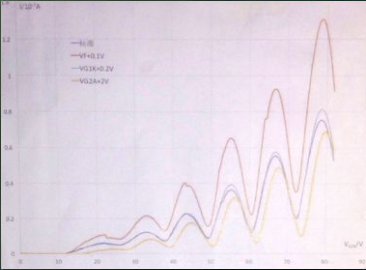
\includegraphics[width=10cm]{lab2151_1.png}
    \caption{四条曲线对比图}
	\end{figure}

\subsection*{5.示波器自动测量}

\begin{figure}[h]
	\centering
		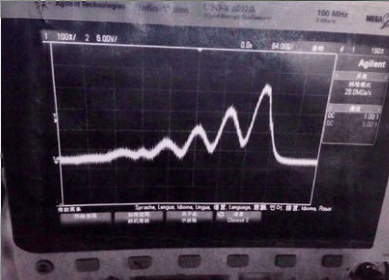
\includegraphics[width=10cm]{lab2151_2.png}
	\end{figure}